\chapter{How to Write Strikingly Well}

This lecture begins with scale rather than technique. The host introduces Lee Child through the astonishing reach of the Reacher books, and then immediately turns that scale into a craft problem: how does one build writing that can move so many readers without dissolving into formula? There is no literal blackboard mathematics here, but there is a real structural mathematics. We move from geography to place, from place to story-constraints, from improvisation to audience design, from audience design to propulsion, and from propulsion to dialogue, beginnings, endings, and the hidden database of reading that makes apparent spontaneity possible.

\section{Frontier Scale and the Narrative Need for America}

The opening move is important. We are not first given a theory of style. We are first given a practical puzzle: why does an English writer, newly fired and needing to make a career, turn to America? Child's answer is layered. Part of it is biographical: he wanted out, and if he could not yet leave physically, he could at least leave narratively. But the deeper answer is formal. The kind of story he wanted to write could not breathe in the geography he was leaving.

We can summarize the contrast schematically:
\begin{equation}
\text{small geography} \Longrightarrow \text{internal / local crime world}, \qquad
\text{frontier-scale geography} \Longrightarrow \text{plausible wandering stranger}.
\end{equation}

This is not a slogan about national taste. It is a claim about plausibility. Barbara Vine and Ian Rankin are invoked as examples of brilliant fiction working inside dense, local, enclosed social worlds. Child wants something else: the older myth of the mysterious stranger, the noble loner who can wander into an isolated community, discover a hidden trouble, and act inside it before the larger world closes in. Britain, in his account, is too crowded, too mutually legible, too tightly packed for that myth to feel natural. America offers the frontier field that makes the plot believable.

The lecture adds a second refinement. America is not merely large; it is also available to him as a place long observed. He had visited the United States repeatedly before emigrating, and he stresses the strange advantage of the outsider's eye: one risks getting details wrong, but one also notices what insiders no longer see.

\subsection{Question \& Answer}

\paragraph{Question.} Why did this fiction have to move to America?

\paragraph{Answer.} Because the desired story-form required it. The mythic wandering stranger is not equally plausible on every map. If everybody knows everybody else's business, the stranger loses his mystery and the community loses its isolation. Child's move to America is therefore not branding in the first instance. It is a narrative solution to a problem of scale. The geography is already functioning as story logic.

A second point enters here and will remain with us throughout the chapter: writing is not presented as pure muse. Child says, quite bluntly, that it is a job. Since he had been fired, the matter was serious. He needed not merely to write, but to make a living and then a career. That pressure does not cheapen the art; it sharpens the design question from the beginning.

\section{Place as Temperature, Key, and Story Physics}

Once the large map is fixed, the host asks the next precise question: how does place become vivid? He offers the usual instruments of description, sound, sight, light, color. Child answers in a much more controlling way. For him, place begins mostly with temperature.

We may write the idea as
\begin{equation}
\text{temperature} + \text{terrain memory} \Longrightarrow \text{story atmosphere} \Longrightarrow \text{action constraints}.
\end{equation}

This is one of the lecture's most valuable formal moves. Place is not scenery pasted onto a pre-existing plot. It is an initial condition. Hot versus cold, hard versus soft, gray mist versus baked dryness: these are not decorative touches. They generate the stage on which some actions feel inevitable and others implausible. The host's phrase ``the physics of the story'' is therefore exactly right.

Child sharpens the point with a musical analogy:
\begin{equation}
G\text{ major} \sim \text{cheerful / upbeat}, \qquad
E\flat \text{ minor} \sim \text{melancholy / down}.
\end{equation}

The analogy matters because it shows the order of construction. A composer chooses a key before the full movement exists. In the same way, Child begins with a vague tonal decision: this book should be hard and cold, or else hot and exposed. Only then does he choose a location already stored in memory: west Texas under brutal heat, or coastal Maine in April, gray and damp. He does not begin by researching a setting specifically for the book. He begins from impressions already accumulated over years.

\subsection{Question \& Answer}

\paragraph{Question.} How do we create place if we are not outlining the story first?

\paragraph{Answer.} We do not wait for plot to tell us where we are. We decide the tonal condition first, and the place follows from that condition. Once the place is chosen, it begins to dictate what can happen there. In that sense, place is not downstream of story. It is one of the engines from which story emerges.

This immediately leads to Child's anti-outline position:
\begin{equation}
\text{outline written} \Longrightarrow \text{story told to self} \Longrightarrow \text{writerly boredom}.
\end{equation}

He insists on the point because, for him, the story is the thing. Writing as wording is not the difficulty; the difficulty is preserving the adventure of discovery. If he outlines even briefly, he has already told himself the tale and wants the next one. Hence the corollary,
\begin{equation}
\text{no external outline} \neq \text{no structure}.
\end{equation}
The meaning of that corollary will unfold only later, when the lecture turns to reading and internalized form.

\section{Improvisation, Reading Formation, and the Series Contract}

The lecture now widens from local method to the reservoir behind the method. Improvisation here is not nakedness. It is improvisation backed by reading, memory, taste, and a long apprenticeship as a reader.

Child gives concrete examples. From Alistair MacLean he learned the art of holding a hero right up to the edge of excess without tipping into the ludicrous. From MacLean's decline he learned a negative lesson as well: success does not excuse boredom or slackness. From John D. MacDonald he learned something harder to state: a book can be utterly addictive even when almost nothing happens on page one. The point is crucial because it warns us against a shallow theory of momentum. Propulsion is not identical with explosions.

The series form is then described from the reader's side. A recurring protagonist gives the audience what Child calls a kind of pre-approval:
\begin{equation}
\text{book}_1 \text{ liked} \Longrightarrow \text{character trusted} \Longrightarrow \text{book}_{n+1} \text{ entered with reduced risk}.
\end{equation}

That equation captures the force of the series contract. The reader still wants a new plot and a new context, but the larger wager has already been lowered. One's old companion is returning. This is why Child keeps returning to the question, ``What did I enjoy as a reader?'' The sequence from readerly appetite to writerly design is never severed.

He also describes the annual rhythm by which a book is actually produced:
\begin{align}
\text{March/April} &:\ \text{book finished},\\
\text{July/August} &:\ \text{self-doubt and apparent depletion},\\
\text{late August} &:\ \text{the first line arrives},\\
\text{September 1} &:\ \text{the next book begins}.
\end{align}

This schedule matters because it shows that imagination is not treated as a random visitation. Child says the imagination is, to some degree, biddable. It can be quieted, and it can be cranked back up. The routine does not replace inspiration, but it gives inspiration a point of re-entry.

At this stage the lecture still sounds anti-planning, but it is no longer romantic. We are beginning to see that improvisation is being stabilized by repetition, by reading history, and by the predictable return of the work itself.

\section{Audience Topology and the Mechanics of Propulsion}

From here the lecture makes one of its strongest formal pivots. Writing is not merely expression. It is not even merely communication. Because Child came through theater and television, he insists that the audience must be included in the calculation. If a show is put on and nobody comes, has the show fully existed as a show? If a book is written and nobody reads it, what kind of existence does it have as a book? This is not crude commercialism. It is a theory of form as transaction.

But the audience is not monolithic. Child's image is the ``rings of Saturn.'' At the center are highly skilled, habitual readers. Farther out are readers who may read one or two books a year. The writer who wants a broad reach must somehow satisfy both.

\begin{figure}[h]
\centering
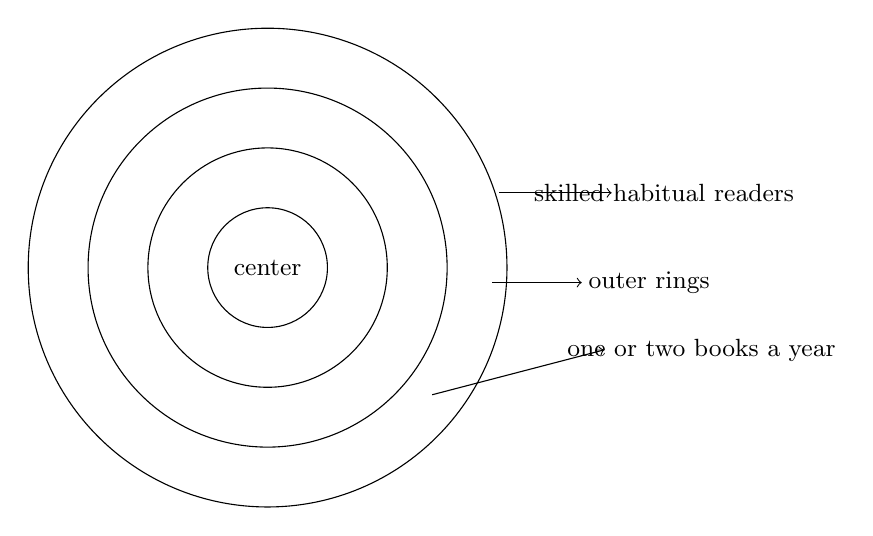
\begin{tikzpicture}[scale=0.95]
\draw (0,0) circle (0.8);
\draw (0,0) circle (1.6);
\draw (0,0) circle (2.4);
\draw (0,0) circle (3.2);
\node at (0,0) {\small center};
\node at (5.3,1.0) {\small skilled habitual readers};
\draw[->] (3.1,1.0) -- (4.6,1.0);
\node at (5.1,-0.2) {\small outer rings};
\draw[->] (3.0,-0.2) -- (4.2,-0.2);
\node at (5.8,-1.1) {\small one or two books a year};
\draw[->] (2.2,-1.7) -- (4.5,-1.1);
\end{tikzpicture}
\end{figure}

The problem can be stated compactly:
\begin{equation}
\text{style must satisfy center} \quad \& \quad \text{style must carry outskirts}.
\end{equation}

\begin{definition}
By \textit{propulsion} we mean the cumulative forward pressure by which one sentence, one paragraph, and one chapter make the next one difficult to resist.
\end{definition}

\subsection{Question \& Answer}

\paragraph{Question.} How do we write for both expert readers and people who barely read at all?

\paragraph{Answer.} Not by writing two different books. The same style must do double duty. At the center it may be appreciated as style. At the edges it must be useful; it must guide, ease, and carry. Child's image is physical and exact: it is as though the writer has a hand gently on the back of the outer-ring reader, pushing that reader through the book without making the pressure felt as pressure.

That is why propulsion becomes a design requirement rather than a mere ornament. Child formulates it at the sentence level:
\begin{equation}
\text{sentence rhythm}_1 \to \text{sentence rhythm}_2 \to \cdots,
\qquad
\Delta p_{\text{sentence}} > 0.
\end{equation}
Here \(p\) is only an editorial name for forward pressure, not the lecturer's notation. The point is simply that each beat should tip slightly ahead of the previous one. The increase is subtle. Child compares it to a pop song whose tempo rises almost imperceptibly as it goes, or to a carnival ride once one has entered the polished tube. The reader need not notice the mechanics. In a sense it is better if the reader does not.

This is also why one of the compliments that most moves him is not an abstract compliment about style but a concrete one: ``I finished it.'' For many readers, especially those in the outer rings, finishing a book is itself an achievement. Propulsion is partly the craft by which the writer helps them reach that point.

\section{Question Engines, Cliffhangers, and Dialogue Illusion}

Once propulsion has been named, the host does exactly the right thing: he refuses to leave it as a grand generality. He asks how it actually works. Does it reside in sentence rhythm alone? Does it appear at chapter endings? Does it depend on opening a question early and delaying the answer? Child's answer is yes. The lecture now becomes openly derivational.

\subsection{Question \& Answer}

\paragraph{Question.} How do questions and rhythm actually pull a reader through a book?

\paragraph{Answer.} By creating a live deficit in knowledge. The audience wants the missing piece, and once that desire is active it can carry attention across the gap. Child learned this in television, and his favorite example is historical. The remote control lowered the cost of leaving. Therefore the need for hooks rose.

We may write the chain as
\begin{equation}
\text{implied question} \Longrightarrow \text{answer withheld} \Longrightarrow \text{reader / viewer retention},
\end{equation}
together with the historical pressure
\begin{equation}
\text{switching cost} \downarrow \Longrightarrow \text{need for sharper hooks} \uparrow.
\end{equation}

The logic is explicit enough to set out as a worked derivation:
\begin{enumerate}
\item In the earlier television world, changing the channel cost effort; the viewer had to rise and do it.
\item That friction created a residue of inertia. The audience might remain through a break simply because leaving was inconvenient.
\item The remote control collapsed that friction.
\item Once channel-switching became almost effortless, inertia no longer protected attention.
\item The producer therefore had to plant a question before the break and postpone the answer.
\item The same device transfers naturally into prose: a chapter closes not merely at a pause, but at an energized question.
\end{enumerate}

Child's deliberately playful demonstration is perfect. He says, in effect, that by 1990 viewers possessed something they did not possess in 1980. The host, and we with him, now want the answer. Only after the desire is active does Child reveal the object: the remote control. This is not just an example of the principle; it is the principle in action.

The lecture then makes a bolder claim. Plotting, in this specific sense, is often exaggerated as a difficulty. Once one knows how to imply a question, the reader's appetite for the answer does much of the work.

The section then turns from question structure to dialogue, but the underlying issue remains the same: how do we engineer motion without making the engineering visible?

\subsection{Question \& Answer}

\paragraph{Question.} How do we make prose feel natural while actually engineering it for motion and emphasis?

\paragraph{Answer.} By refusing to mistake literal transcription for realism. Real speech is chaotic. Written dialogue must therefore be artificial, but artificially tuned in such a way that the reader experiences it as natural.

Child states the point with unusual bluntness:
\begin{equation}
\text{real speech} \neq \text{written dialogue},
\qquad
\text{written dialogue} = \text{structured artifice that must feel natural}.
\end{equation}

Real speech is full of false starts, fillers, jumps of subject, and dead space. Yet if we copied all of that, the page would become unreadable. So the craft problem is not to reproduce speech, but to reproduce the illusion of speech. Rhythm does the work. Stress does the work. Selective repetition does the work.

The host's train anecdote gives us a small worked example:
\begin{equation}
\text{``I need my money''}, \qquad \text{``I lost my money''}
\Longrightarrow
\text{need / lost / money become stress points.}
\end{equation}

We can unpack the mechanism in a few short steps:
\begin{enumerate}
\item The noun \emph{money} is repeated, so it persists in the ear.
\item The surrounding filler drops away under emotional pressure.
\item The verbs \emph{need} and \emph{lost} carry the changing charge.
\item The sentence sounds immediate and spoken precisely because it has been simplified and rhythmically focused.
\end{enumerate}

Child prefers not to depend too heavily on italics, since a page peppered with italics turns emphasis into typographical noise. Better to shape the line so that its rhythm lands on the right word by itself. That is the deeper continuity between the sentence-level propulsion of the previous section and the dialogue problem here: both depend on controlled pressure.

\section{Beginnings, Endings, and the Monster Outline in the Head}

The lecture now broadens again. It begins at a surprisingly large scale: when should a person begin writing at all? Child's answer is that most would-be writers are too early. Talent and enthusiasm are present, but content is thin. One should read, live, accumulate, and only later begin in earnest. At the macro scale, then, beginnings and endings belong to a life. At the scale of the book, however, the rules are cleaner.

They can be written in two short equations:
\begin{equation}
\text{do not start when the earth cooled} \Longrightarrow \textit{in medias res},
\end{equation}
\begin{equation}
\text{story over} \Longrightarrow \text{book over}.
\end{equation}

The first rule attacks the novice tendency to smother the present action beneath formation story and biography. We do not need everything first. We need something alive now. The second rule is equally severe. One stops not at a page target but at closure. Child gives the vivid example of thinking he had another chapter and a half to write, and then suddenly realizing that the book was already done.

The section also revisits television from another angle. Once television became a parallel activity rather than a fully concentrated activity, producers developed a triple redundancy: tell them that we are going to tell them, tell them, and then tell them that we told them. Child became wary of carrying too much of that habit into his novels. He began instead to experiment with leaving the conclusion unassembled, letting the information lie in plain sight while trusting the reader to perform the final integration.

\subsection{Question \& Answer}

\paragraph{Question.} If there is no written outline, where does structure come from?

\paragraph{Answer.} From the enormous internal store built by reading. This is the lecture's answer to the objection that improvisation must mean shapelessness. Child agrees that he makes no plan on paper. But he also says that by reading tens of thousands of books he has, in effect, acquired a vast internal database of available plots, cliffhangers, characters, and structures.

The idea may be expressed as
\begin{equation}
\text{tens of thousands of books read} \Longrightarrow \text{internal database of plots, characters, cliffhangers, structures}.
\end{equation}

So the stronger reconstruction is
\begin{equation}
\text{improvisation} + \text{massive prior reading} \Longrightarrow \text{implicit structural control}.
\end{equation}

This is why Child can say, with no contradiction on the deeper level, that he has no outline and also that he has a ``monster outline.'' The outline is simply not externalized. It is distributed through memory, habit, and taste.

His late formulation is beautifully economical:
\begin{equation}
\text{books written per year} \ll \text{books read per year}.
\end{equation}
Therefore the writer is, in a very literal sense, more reader than writer. Structure is not absent. It has been absorbed.

\section{Violence, Character Shorthand, and the Limits of Teaching}

The final movement of the lecture keeps returning to the same master theme: fiction works not by literal reproduction but by stylized selection. Violence is the clearest example. Child says outright that violence in narrative is, again, an illusion. Real violence is typically brief, ugly, and followed by significant after-effects. The stylized back-and-forth of screen fighting is largely unreal.

So why does the reader want it? The answer is a paradox:
\begin{equation}
\text{civilized commitment to due process} + \text{private retaliatory desire}
\Longrightarrow
\text{fictional violence as release}.
\end{equation}

The reader believes in law, in rights, in safeguards, in the restraint required by civilization. But the same reader also knows the sudden desire to strike back when wronged. Fiction offers a release valve. It permits the retaliatory fantasy to occur inside a domain explicitly understood to be unreal.

This late section also clarifies the economy of characterization. Clothing and teeth are treated as fast visual operators. A ponytail with double denim, or careful lace-up shoes with pleated chinos, or the shape of someone's teeth: each of these can act as a shorthand reference that quickly places a person inside a social type. The point is not that character reduces to costume. The point is that fiction often needs efficient signals.

\subsection{Question \& Answer}

\paragraph{Question.} Can writing actually be taught, or only learned through long exposure?

\paragraph{Answer.} Child's answer is discriminating. Much of the business around writing can certainly be taught: agents, publishers, mistakes to avoid. But the central art is not, in his view, teachable in the straightforward classroom sense. It may nevertheless be learnable. One can read for years and gradually absorb what one could not have been directly handed as a rule.

That answer fits everything that has come before. Dialogue is learned by listening. Structure is learned by reading. Character is sharpened by watching people. Even cultural conditions enter the matter. Child's closing comments on Scotland and Ireland are not a digression. Scotland, in his telling, develops an alternative culture against the pull of centralized power. Ireland gives one something else: a chance. In the pub, if one starts a story well enough, the room will give one a few seconds of hearing. That small allowance matters. It trains the storyteller to seize attention, justify it quickly, and keep it.

The lecture ends, then, not with a technique but with a culture of attention. To be heard, one must have something to say; to say it well, one must have lived, read, listened, and learned how to hold the room.

\section{Summary}

The chapter's sequence is itself the lesson. We begin with scale, because scale immediately forces the question of design. From there we move to geography, and from geography to place as temperature, key, and constraint. Improvisation then turns out not to be the absence of form but the deployment of an internalized form built by reading. Audience design leads to propulsion; propulsion leads to question-making; question-making leads to dialogue, chapter endings, and immersion. The late material on violence, character shorthand, and teachability does not depart from the earlier themes. It confirms them. Writing here is neither pure art nor mere labor, but both at once:
\begin{equation}
\text{writing as art} = 100\%, \qquad \text{writing as job} = 100\%.
\end{equation}
Child calls that mathematically impossible, and that is exactly why it is the right closing formula for the lecture.